\documentclass[default]{beamer}
\setbeamertemplate{navigation symbols}{}

\usetheme{CambridgeUS}
\useoutertheme{infolines}
%\usecolortheme{crane}

\usepackage{cmap}							% Поддержка поиска русских слов в PDF (pdflatex)
\usepackage[utf8]{inputenc}					% Выбор языка и кодировки
\usepackage[english, russian]{babel}
\usepackage{csquotes}
\usepackage{algorithm}
\usepackage{algpseudocode}

\usepackage[
	language=auto,
	autolang=other,
	backend=biber,
	style=authortitle,
	sorting=ydnt
]{biblatex}
\addbibresource{dqn.bib}
				
\DeclareSourcemap{
	\maps[datatype=bibtex, overwrite]{
		\map{
			\step[fieldset=langid, fieldvalue=english]
			\step[fieldset=doi, null]
			\step[fieldset=issn, null]
			\step[fieldset=isbn, null]
			\step[fieldset=url, null]
			\step[fieldsource=language, fieldset=langid, origfieldval]
		}
	}
}


\graphicspath{{../../images/misc/}} 			% Пути к изображениям

\makeatletter
\setbeamertemplate{footline}
{
	\leavevmode%
	\hbox{%
		\begin{beamercolorbox}[wd=.333333\paperwidth,ht=2.25ex,dp=1ex,center]{author
				in head/foot}%
			\usebeamerfont{author in
				head/foot}\insertshortauthor~~\beamer@ifempty{\insertshortinstitute}{}{(\insertshortinstitute)}
		\end{beamercolorbox}%
		\begin{beamercolorbox}[wd=.333333\paperwidth,ht=2.25ex,dp=1ex,center]{title in
				head/foot}%
			\usebeamerfont{title in head/foot}\insertshorttitle
		\end{beamercolorbox}%
		\begin{beamercolorbox}[wd=.333333\paperwidth,ht=2.25ex,dp=1ex,right]{date in
				head/foot}%
			\usebeamerfont{date in head/foot}\insertshortdate{}\hspace*{2em}
			\insertframenumber{}\hspace*{2ex} 
		\end{beamercolorbox}
	}%
	\vskip0pt%
}


\renewcommand*{\bibfont}{\tiny}
\setlength\bibitemsep{-5pt}

\begin{document}
	
	\title[DQN]{Глубокое обучение с подкреплением играх Atari}
	\author[Панов]{Александр Панов}
	\institute[ИСА РАН]{ИСА РАН}
	\date{30 июня 2016~г.} 
	
	\begin{frame}
		\titlepage
	\end{frame}
		
	\begin{frame}
		\frametitle{Постановка задачи}

		\begin{columns}
			\begin{column}{0.7\textwidth}
				\begin{itemize}
					\item Внешняя среда (стохастическая) $\mathcal E$
					\item Дискретное время $t\in\mathbb N$
					\item Действия $a_t \in \mathcal A=\{1,..,K\}$
					\item Наблюдаемое изображение $x_t\in\mathbb R^d$
					\item Вознаграждение (изменение счета) $r_t$
					\item Описание текущего состояние через последовательность действий и наблюдений:
					\[
					s_t = x_1,a_1,x_2,\dots,a_{t-1},x_t
					\]
					\item Цель агента - взаимодействовать со средой, выбирая действия таким образом, чтобы максимизировать будущее вознаграждение.
				\end{itemize}
			\end{column}
			\begin{column}{0.3\textwidth}
				\centering
				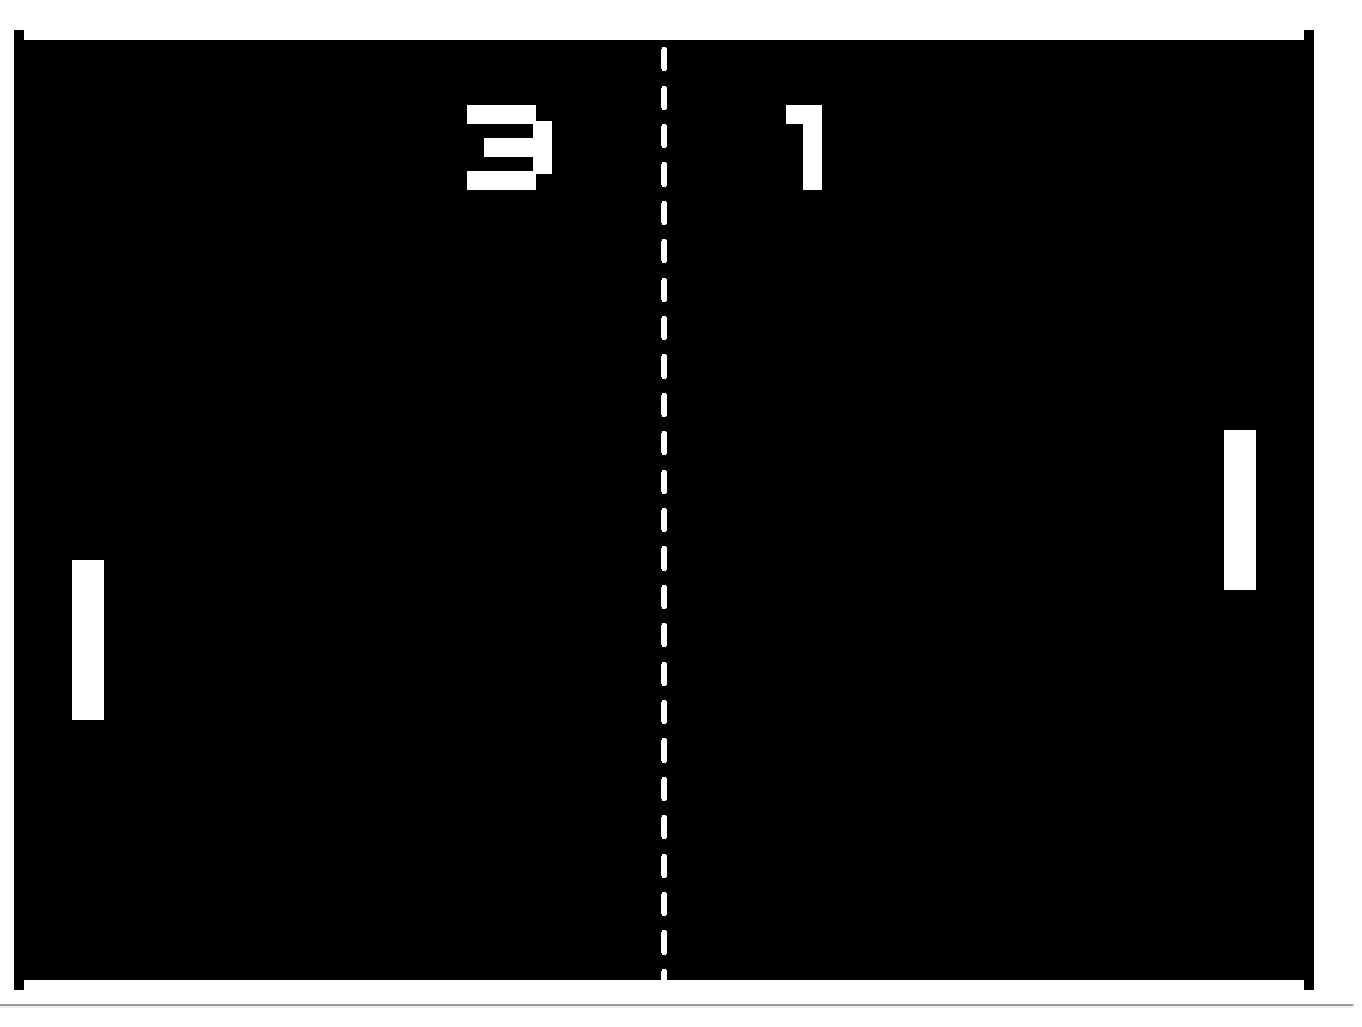
\includegraphics[width=\textwidth]{ponggame}
			\end{column}
		\end{columns}
		
		\par\medskip
		\nocite{*}
		\printbibliography
	\end{frame}
	

	\begin{frame}	
		\frametitle{Q-обучение}
		\small
		Будущее вознаграждение спадает со временем 
		\[
			R_t=\sum_{t'=t}^T \gamma^{t'-t}r_{t'},
		\]
		$T$ - время окончания игры.
		\par\medskip
		Оптимальное значение функции оценки действий
		\[
			Q^*(s,a) = \max_\pi\mathbb E\big[R_t|s_t=s,a_t=a,\pi\big],
		\]
		$\pi$ - стратегия выбора действия.		
		\par\medskip
		Уравнение Беллмана
		\[
			Q^*(s,a) = \mathbb E_{s'\sim\mathcal E}\big[r+\gamma\max_{a'}Q^*(s',a')\big|s,a\big],
		\]
		откуда следует итеративный процесс вычисления оптимального значения $Q_i\rightarrow Q^*$:
		\[
			Q_{i+1}(s,a) = \mathbb E\big[r+\gamma\max_{a'}Q_i(s',a')\big|s,a\big].
		\]
	\end{frame}	

	
	\begin{frame}	
		\frametitle{Q-обучение}
		\small
		Для придания обобщающей силы используют аппроксимации
		\[
			Q(s,a;\theta)\approx Q^*(s,a).
		\]
		\par\medskip
		При использовании в качестве аппроксиматора нейронной сети получаем Q-сеть с функцией потерь
		\[
			L_i(\theta_i)=\mathbb E_{s,a\sim\rho(\cdot)}\big[(y_i-Q(s,a;\theta_i)^2)\big],
		\]
		где $\rho(s,a)$ - распределение вероятности по последовательностям $s$ и действиям $a$, а
		\[
			y_i=\mathbb E_{s'\sim\mathcal E}\big[r+\gamma\max_{a'}Q(s',a';\theta_{i-1})\big|s,a\big].
		\]
		\par\medskip
		Соответствующий градиент для SGD
		\[
			\nabla_{\theta_i}L_i(\theta_i)=\mathbb E_{s,a\sim\rho(\cdot);s'\sim\mathcal E}\bigg[\big(r+\gamma\max_{a'}Q(s',a';\theta_{i-1})-Q(s,a;\theta_i)\big)\nabla_{\theta_i}Q(s,a;\theta_i)\bigg]
		\]
		
	\end{frame}	
	
	\begin{frame}
		\frametitle{Q-обучение, переигровка (experience reply)}
		
		Model-free, off-policy: $a=\max_a Q(s,a;\theta)$.
		\par\medskip
		Каждый момент сохраняется опыт (прецедент) $e_t=(s_t,a_t,r_t,s_{t+1})$ в память переигровок $\mathcal D=e_1,\dots,e_N$.
		
		\par\medskip
		Архитектура сети:
		\begin{itemize}
			\item Входное цветное изображение 210x160 ужимается до серых тонов 84x84 (функция $\phi$).
			\item Функция $\phi$ применяется к последним 4 кадрам (4 изображения).
			 \item Первый скрытый слой - 16 сверточных фильтров 8x8 с шагом 4.
			 \item Второй скрытый слой - 32 сверточных фильтра 4x4 с шагом 2.
			 \item Последний скрытый слой - полносвязный (256 rectifier units).
			 \item Выходной слой - полносвязный линейный на выход для каждого возможного действия (4--18).
		\end{itemize}
										
	\end{frame}											
										
	\begin{frame}
		\frametitle{DQN с переигровкой}
		\small
			\begin{algorithmic}[1]
				\State Initialize replay memory $\mathcal D$ to capacity $N$ 
				\State Initialize action-value function $Q$ with random weights 
				\ForAll{episode = $1,M$}
					\State Initialise sequence $s_1 = \{x_1\}$ and preprocessed sequenced $\phi_1 = \phi(s_1)$ 
					\ForAll{$t = 1,T$}
						\State With probability $\epsilon$ select a random action $a_t$ 
						\State otherwise select $a_t = \max_a Q^*(\phi(s_t),a; \theta)$
						\State Execute action $a_t$ in emulator and observe reward $r_t$ and image $x_{t+1}$
						\State Set $s_{t+1} = s_t, a_t,x_{t+1}$ and preprocess $\phi_{t+1} = \phi(s_{t+1})$
						\State Store transition $(\phi_t, a_t, r_t,\phi_{t+1})$ in $\mathcal D$ \State Sample random minibatch of transitions $(\phi_j, a_j, r_j,\phi_{j+1})$ from $\mathcal D$
						\State Set 
						\[
							y_j =\begin{cases}
								r_j& \text{for terminal }\phi_{j+1} \\
								r_j +\gamma\max_{a'}Q(\phi_{j+1},a';\theta)& \text{for non-terminal }\phi_{j+1}
							\end{cases}		
						\]
						\State Perform a gradient descent step on $(y_j-Q(\phi_j, a_j;\theta))^2$
					\EndFor 
				\EndFor
			\end{algorithmic}
	\end{frame}											

%	\begin{frame}
%		\frametitle{Цели курса}
%		
%		\begin{columns}
%			\begin{column}{0.5\textwidth}
%				
%			\end{column}
%			\begin{column}{0.5\textwidth}
%				\begin{figure}
%					
\includegraphics[width=\textwidth]{logo}
%				\end{figure}
%			\end{column}
%		\end{columns}
%	\end{frame}
	%	\begin{frame}
	%		\frametitle{Цели курса}
	%		
	%		\begin{itemize}
	%			\item
	%		\end{itemize}
	%	\end{frame}
	
\end{document}
	
	
